\section{Number Representations}
\subsection{Types}
\paragraph{Base Two}
Numbers in computers are represented in binary, base two, format. Normally, our normal understanding of numbers is in Base Ten. \[3 = 1 \times 10^0\] but this can also be represented in Base Two \[3_10 = 11_2 = 1 \times 2^1 + 1 \times 2^0\]. In terms of integers at least, this means that the maximum size we can represent in $n$ bits is \[2^n - 1\] so a 32-bit value is, at most, $2^{32} - 1$.
\paragraph{Representations}
Ofcourse, this method of representation using twos also works for decimals, but where in a byte do we store decimals? In the fixed point representation of real numbers, the decimal is implied. For example, assuming a 16-bit piece of memory, we imply that the integer portion will cover the first 8 bits and the decimal portion the remaining 8 bits. As such, the computer will recognize the values with no manual decimal placed.
Modern computers now use the floating point representation. \[V = M \times 2^E\] Floating point uses a mantissa $M$ and an exponent $E$ to store its values. Part of the bits, for example 4 bits in an 8-bit system, are used to store the mantissa and the rest represent the exponent. In an 8 bit system as a result, you can represent a value like 112 as \[01110111 \rightarrow 0.111 \times 2^{0111}\]
\paragraph{Negative Value}
Negative values are represented using something we like to call Two's Complement. What this simply means is, the left-most bit is "0" for the positive variant. We know that each value we can represent should have a value in the same field that, when added together, form $0$. We represent this negative value by inverting every bit and adding 1 to the LSB. \[ 0101 \rightarrow 1011\]. The system reads the left-most bit as a 1, so we know its negative, the rest follows.

\subsection{Arithmetic}
\begin{figure}[!htb]
	\center{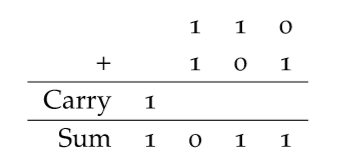
\includegraphics[width=5cm]
		{csa/adding}}
	\caption{\label{fig:adding} Arithmetic example for base 2}
\end{figure}
Adding bits works the same as adding and subtracting the numbers in base 10. For example, if we were to add $0110$ and $0101$, the result would be $1011$ as seen by the figure. When our column adds to a total of 2, a one is carried on column to the right and the 2 becomes a 0. If the total becomes 3, a 1 is still carried, but the column becomes a 1.
For subtraction, you can add the base value and the two's compliment of the other value. This simplifies the process greatly.

\section{Logic}
\subsection{Logic Gates}
The basic building block of our CPUs today are transistors. Transistors are made up of three parts, a gate, a source, and a drain. They are used in circuits; it is enough to understand that they are switches that are controlled by the gate voltage.
Transistors process bits (0 voltage and $>$ 0 voltage). The output changes based on how the circuit is built. For example, we have the NOT gate which takes a signal and inverts it on output. For simplicity, gates are drawn in an abbreviated form as seen in Figure \ref{fig:gates}.
\begin{figure}[!htb]
	\center{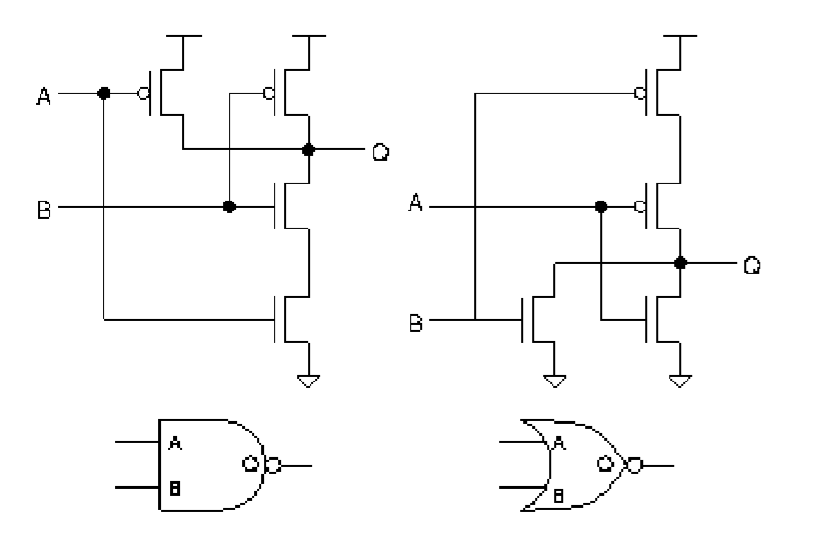
\includegraphics[width=9cm]
		{csa/gates}}
	\caption{\label{fig:gates} NAND and NOR gates}
\end{figure}
If you've done Minecraft Redstone, you might find yourself at home on this section. Sadly real life is a little more complicated.
\paragraph{Combination Logic} A general term for blocks of digital logic which contain no kind of memory. For each $n$ inputs, there are $2^n$ possible output states. Each of these outputs can be represented by a basic boolean algebra (eg. $A\wedge B$) and written into a circuit as such.
\subsection{ALU}
multiplexer
adders/halfadder

\section{Architecture}
\subsection{von Neumann}
memory, load/store unit, registers, instruction register, alu, program counter, 

\subsection{cycles}
cpu cycles
instruction cycle: fetch-decode-execute

\section{MIPS Microarchitecture}
\subsection{Datapath}
instruction fetch (r-type)
load/store (i-type)
multiplexing
integrating them
jump instruction

\subsection{Controls}
cpu controls
alu control
main control

\section{Optimisation}
cache
locality
associativity
c/c++ matrices example